% !TEX TS-program = pdfLaTeX+shellescape
% !TEX encoding = UTF-8 Unicode

\documentclass{standalone}
\usepackage{pgfplots}
\pgfplotsset{compat=1.18}

\begin{document}
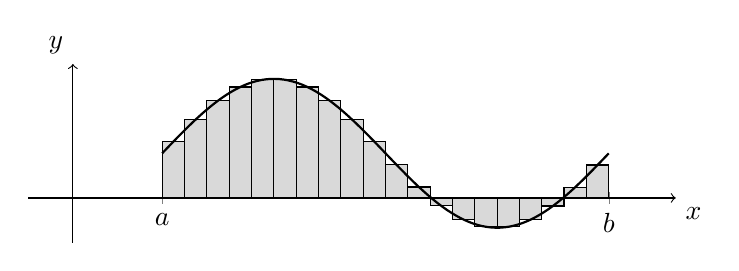
\begin{tikzpicture}
\begin{axis}[
axis lines = middle,
unit vector ratio=1 1, 
% axis equal=false,
scale=1.2, 
xmin=-0.1, xmax=1.35, ymin=-0.1, ymax=0.30, 
% grid = major,
xtick={0.2,1.2},
ytick={0},
xticklabels = {$a$, $b$},
yticklabels = {},
xlabel=$x$,
ylabel=$y$,
xlabel style={below right},
ylabel style={above left},
axis line style = {->},
declare function={
    myfunc(\x,\a) = (sin(deg(2*pi*(\x-\a)))+0.6)/6;
}
]

\pgfmathsetmacro{\a}{0.2} 
\pgfmathsetmacro{\b}{1.2}
\pgfmathtruncatemacro{\Nsub}{20} 
\pgfmathsetmacro{\h}{(\b-\a)/\Nsub}

\pgfplotsforeachungrouped \i in {0,...,\Nsub-1}{
    \pgfmathsetmacro{\xleft}{\a+\i*\h}
    \pgfmathsetmacro{\xright}{\a+(\i+1)*\h} 
    \pgfmathsetmacro{\xmid}{\a+(\i+0.5)*\h}
    \pgfmathsetmacro{\height}{myfunc(\xmid,\a)} 
    \edef\doplot{\noexpand 
        \fill[gray!30] (axis cs:{\xleft},{0}) rectangle (axis cs:{\xright},{\height}); 
    }
    \doplot
    \edef\doplot{\noexpand 
        \draw (axis cs:{\xleft},{0}) rectangle (axis cs:{\xright},{\height});
    }
    \doplot
}

\addplot [style=thick, domain=0.2:1.2, samples=100] {(sin(deg(2*pi*(x-0.2)))+0.6)/6};

\end{axis}
\end{tikzpicture}


\end{document}